\documentclass{sintefbeamer}

% packages, font, color, and newcommands
\usepackage{amsfonts, amsmath, oldgerm, lmodern, bm}
% \usepackage[font={footnotesize}]{caption}
\usepackage{natbib}
\usepackage{url}
\usepackage{tikz}
\usepackage{amssymb}
\usepackage{amsmath}
\usepackage{amsthm}
\usepackage{mathrsfs}
\usepackage{empheq}
\usepackage{mdframed}
\usepackage{bm}
\usepackage{animate}
\usepackage{xcolor,colortbl}
\usepackage{graphicx}
\usepackage{stmaryrd}
\usepackage{amsmath}
\usepackage{animate}
\usepackage{array}
%\usepackage{cancel}

\tikzset{  node distance=3cm and 5cm,
every node/.style={align=center, font=\sffamily},
box/.style={ rounded corners, minimum width=3.5cm, minimum height=1cm, text centered,fill=sintefblue!15},
arrow/.style={-{Latex}, thick}}
\bibliographystyle{apalike}

\useoutertheme{miniframes}
\usefonttheme{serif}

\usetikzlibrary{arrows.meta,
                chains,
                calc,
                positioning,
                shapes.geometric,
                backgrounds}

\title{The closure problem in dispersed two-phase flows: How 19th-century mathematical approaches can be as efficient as modern numerical simulations}
%\subtitle{Presentation VS 6 2025, Solaize France}

\author
{\href{http://basilisk.fr/sandbox/fintzin/Rising-Suspenion/RS.c}
{N. Fintzi\footnote{IFP \'Energies Nouvelles, France}$^{,2}$},  
S. Popinet\footnote{Sorbonne Universit\'e, France} and
\underline{JL. Pierson$^1$}}


\titlebackground{image/800good.png}

% document body
\addtobeamertemplate{navigation symbols}{}{%
    \usebeamerfont{footline}%
    \usebeamercolor[fg]{footline}%

    \insertframenumber/\inserttotalframenumber
}


% \includeonlyframes{current}


\begin{document}

{\setbeamertemplate{headline}{}
% \setbeamertemplate{footline}{}
\setlength{\headheight}{0pt}
\maketitle
}

\section{Context}


\begin{frame}
  \frametitle{Why studying dispersed two-phase flows ? }
  \centering
  {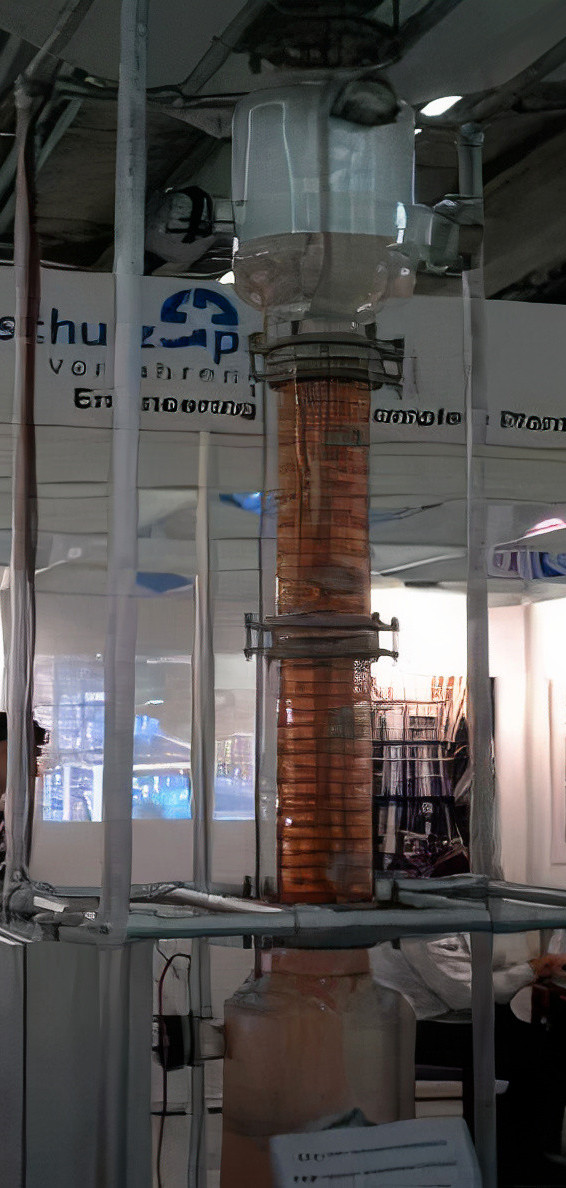
\includegraphics[height=0.3\textwidth]{image/liq-liq_LE_auto_x5.jpg}}
  \uncover<2->{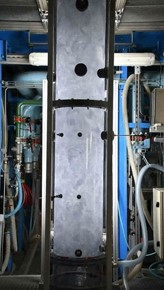
\includegraphics[height=0.3\textwidth]{image/Image2.jpg}}
  \uncover<3->{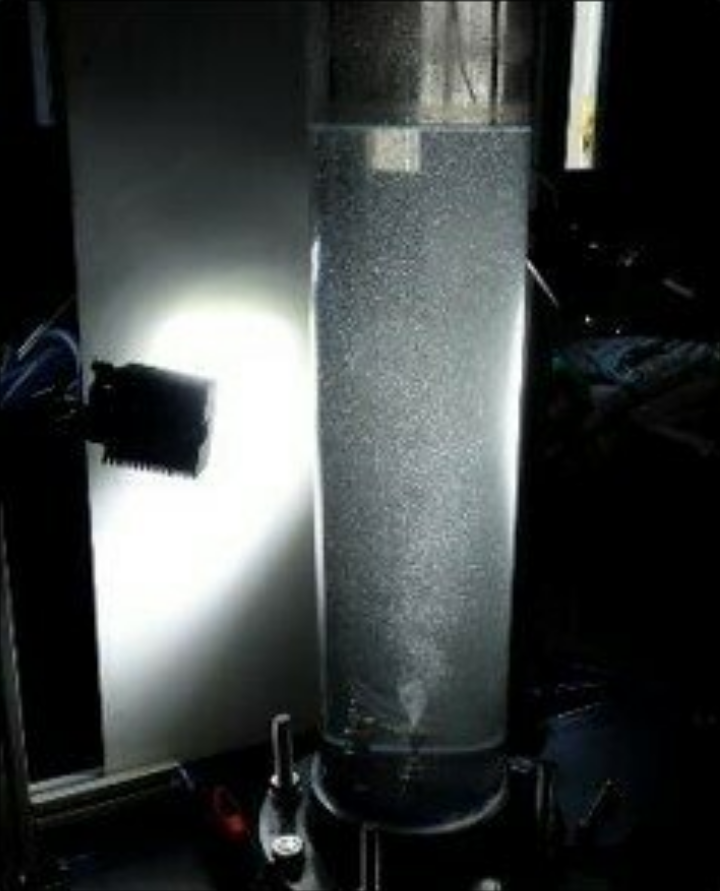
\includegraphics[height=0.3\textwidth]{image/flo.png}}
  %\uncover<4->{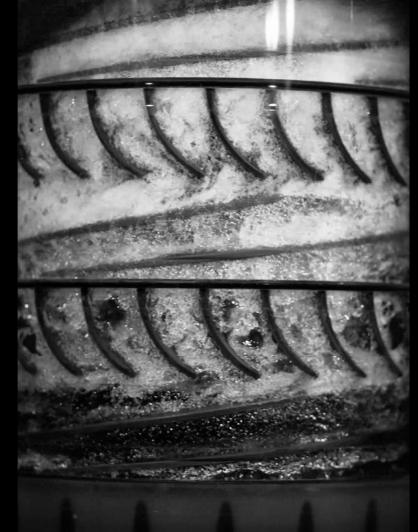
\includegraphics[height=0.3\textwidth]{image/Image4.png}}
  \begin{itemize}
    \item<1-> Liquid-liquid separation processes
    \item<2-> Bubbles columns
    \item<3-> Flotation columns
    %\item<4-> Pneumatic transports
    %\item<4-> Multiphase pumps
    %\item<5-> And other\ldots
  \end{itemize}
  Buoyancy dominated flows (with turbulence) : \\ $ Re_L \gg  1$, $ 0.1 \leq Re _p \leq 200 $, $0 \leq \rho_p/\rho_f \leq 1.5,0.01 \leq \mu_p /\mu _f (=\lambda) \leq 10$
\end{frame}


\begin{frame}
  \frametitle{Problem ! \uncover<3->{Upscaling ?} }
      \centering
      \setbeamercovered{transparent=10}

      \begin{tikzpicture}
        \node (img) at (0,0) {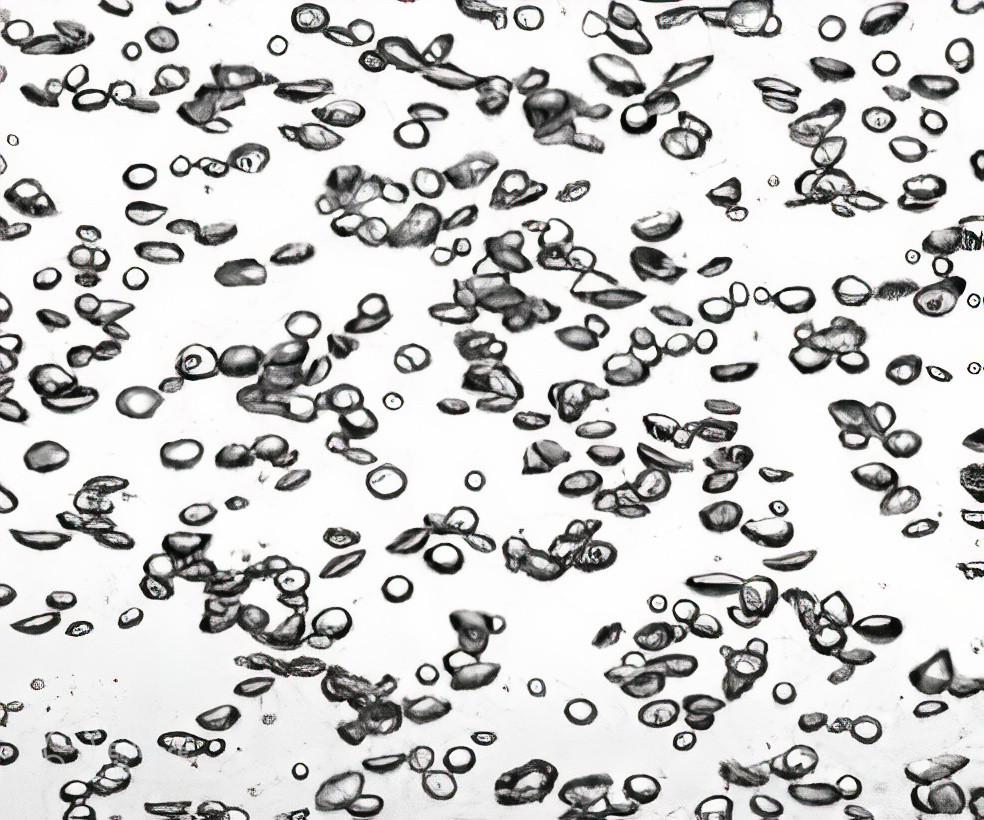
\includegraphics[height=0.25\textwidth]{image/bubbles_4x.jpg}};
        \node[above] (title1) at (0,0.125\textwidth) {\textbf{Local description} \citep{Dung_Waasdorp_Sun_Lohse_Huisman_2023}};
        \uncover<3->{
        \node[text width=6cm] (itm) at (0.55\textwidth,0) {
          \begin{itemize}
            \item Volume fraction of droplets ?  
            \item Mean velocity of each phase ? 
            \item \ldots
          \end{itemize}
          };
          \node[above] (title2) at (0.55\textwidth,0.125\textwidth) {\textbf{Macroscopic description}};
        \draw[arrow,very thick] (img) -- (itm)node[midway,above]{Upscaling};
        }
        \uncover<1->{
          \node[yshift=-3em,box,text width=5cm] (eq1) at (0,-0.125\textwidth) {Navier-Stokes equations and Newton second-law of motion};
          \draw[arrow](img) -- (eq1);
        }
        \uncover<4>{
          \node[yshift=-3em,box] (eq2) at (0.55\textwidth,-0.125\textwidth) {\underline{Averaged} Navier-Stokes equations};
          \draw[arrow](itm) -- (eq2);
        }
      \end{tikzpicture}

      \vfill

      \uncover<2->{
      $\to$\textbf{Problem :} For large number of particles computations are unfeasible !
      }
\end{frame}


%\begin{frame}
%  {Mathematical modeling of dispersed two-phase flows }
    
  
%  \begin{tikzpicture}
  
  
%  \node[box] at (0,3)(lagrangian) {Lagrangian description of droplets \\ $\ddt (m_i\textbf{u}_i) = \sum \textbf{F}_i$};
%  \node[box] at (8,3)(Eulerian) {Eulerian description of the continuous phase \\ $\div\textbf{u}= 0$\\ $\rho (\pddt + \textbf{u}\cdot\grad)\textbf{u} = \div\bm\sigma + \rho\textbf{g} $};
%  \uncover<2->{
%  \node[box] at (0,0)(kinetic) {``Kinetic Theory''-like models \\(Chapman \& Cowling 1990)};
%  \node[box] at (8,0)(twofluid) {Two-Fluid formulation \\(Drew 1983)};
%  \draw[arrow] (lagrangian) -- (kinetic) node[midway, right] {Statistical averaging};
%  \draw[arrow] (Eulerian) -- (twofluid) node[midway, right] {Statistical  averaging};
%  }
%  \uncover<3>{
%  \node[box] at (4,-2.7)(unify)  {Hybrid Multiphase Flow model (Lhuillier 1992, Zhang \& Prosperetti 1994)};
%  \draw[arrow] (twofluid) -- (unify);
%  \draw[arrow] (kinetic) -- (unify);
%  \draw[arrow] (twofluid) -- (unify);
  %\node[below =0.5cm of kinetic, text width=4.5cm] (desc1) {\textit{Describes the mean particle trajectories}};
  %\node[below =0.5cm of twofluid, text width=4.5cm] (desc2) {\textit{Models the average continous phases behaviour}};
%  }
%  \end{tikzpicture}
  
%\end{frame}




% \section{Lagrangian's description of fluid particles for kinetic-theory}
\section{Averaged equations}
\section*{}

\begin{frame}
  {Mathematical modeling of dispersed two-phase flows }
    
  
  \begin{tikzpicture}
  
  
  \node[box] at (0,3)(lagrangian) {Lagrangian description of droplets \\ $\ddt (m_i\textbf{u}_i) = \sum \textbf{F}$};
  \node[box] at (8,3)(Eulerian) {Eulerian description of the continuous phase \\ $\div\textbf{u}= 0$\\ $\rho (\pddt + \textbf{u}\cdot\grad)\textbf{u} = \div\bm\sigma + \rho\textbf{g} $};
  \uncover<2->{
  \node[box] at (0,0)(kinetic) {``Kinetic Theory''-like models \\ (Chapman 1917, Simonin 1996)};
  \node[box] at (8,0)(twofluid) {Two-Fluid formulation \\ (Drew 1983)};
  \draw[arrow] (lagrangian) -- (kinetic) node[midway, right] {Statistical averaging};
  \draw[arrow] (Eulerian) -- (twofluid) node[midway, right] {Statistical  averaging};
  }
  \uncover<3>{
  \node[box] at (4,-2.7)(unify)  {Hybrid Multiphase Flow model (Lhuillier 1992, Zhang et Prosperetti 1994)};
  \draw[arrow] (twofluid) -- (unify);
  \draw[arrow] (kinetic) -- (unify);
  \draw[arrow] (twofluid) -- (unify);
 % \node[below =0.5cm of kinetic, text width=4.5cm] (desc1) {\textit{Describes the mean particle trajectories}};
 % \node[below =0.5cm of twofluid, text width=4.5cm] (desc2) {\textit{Models the average continous phases behaviour}};
  }
  \end{tikzpicture}
  
  \end{frame}

\begin{frame}
  {Fluid averaged equations }
  \begin{align*}
    &\pddt (\phi_f \rho_f)  
    + \div (
        \phi_f \rho_f\textbf{u}_f
    )
    = 
    0,\\
    &
    \phi_f \rho_f (\pddt + \textbf{u}_f\cdot \grad)\textbf{u}_f
    = 
    \underbrace{\phi_f\div \bm\Sigma^\text{f}}_\text{Mean Newtonian stress}+
    \underbrace{\div \bm\sigma^\text{eff}}_\text{Effective stress}
    + \underbrace{\phi_f \rho_f \textbf{g} }_\text{Buoyancy}
    \only<1>{- \underbrace{\pSavg{{\bm{\sigma}_f' \cdot \textbf{n}}}}_\text{Mean force}}
    \only<2>{\textcolor{sintefcyan}{- \underbrace{\pSavg{{\bm{\sigma}_f' \cdot \textbf{n}}}}_\text{Mean force}}}
  \end{align*}
  \underline{Effective stress: } 
  \begin{equation*}
    \bm{\sigma}_f^\text{eff}
    =
    \only<1>{- \underbrace{\avg{\chi_f\rho_f\textbf{u}_f'\textbf{u}_f'}}_\text{Reynolds Stress}}
    \only<2>{\textcolor{orange}{- \underbrace{\avg{\chi_f\rho_f\textbf{u}_f'\textbf{u}_f'}}_\text{Reynolds Stress}}}
    \only<2>{\textcolor{orange}{+ \underbrace{ {\pSavg{{\left[\textbf{r}\bm{\sigma}_f' \cdot \textbf{n}-\mu_f(\textbf{u}_f'\textbf{n} +\textbf{n}\textbf{u}_f')\right]}}}}_\text{First moment} }}
    \only<1>{+ \underbrace{ {\pSavg{{\left[\textbf{r}\bm{\sigma}_f' \cdot \textbf{n}-\mu_f(\textbf{u}_f'\textbf{n} +\textbf{n}\textbf{u}_f')\right]}}}}_\text{First moment} }
    -\underbrace{\div [\ldots]}_\text{higher moments}
  \end{equation*}

\uncover<2>{
$\to$ Solved quantities: $\phi_f, \textbf{u}_f, \textbf{u}_p, \ldots$.

$\to$ We are looking for $\texttt{CLOSURE TERMS} = f(\phi_f, \textbf{u}_f, \textbf{u}_p, \ldots)$.}
\end{frame}

\begin{frame}
  How to close the problem ?
\begin{figure}
  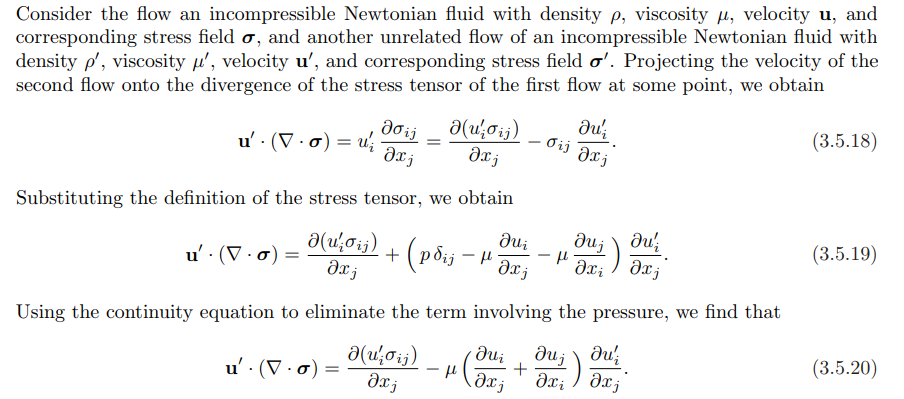
\includegraphics[width=4cm]{image/reciprocal}
  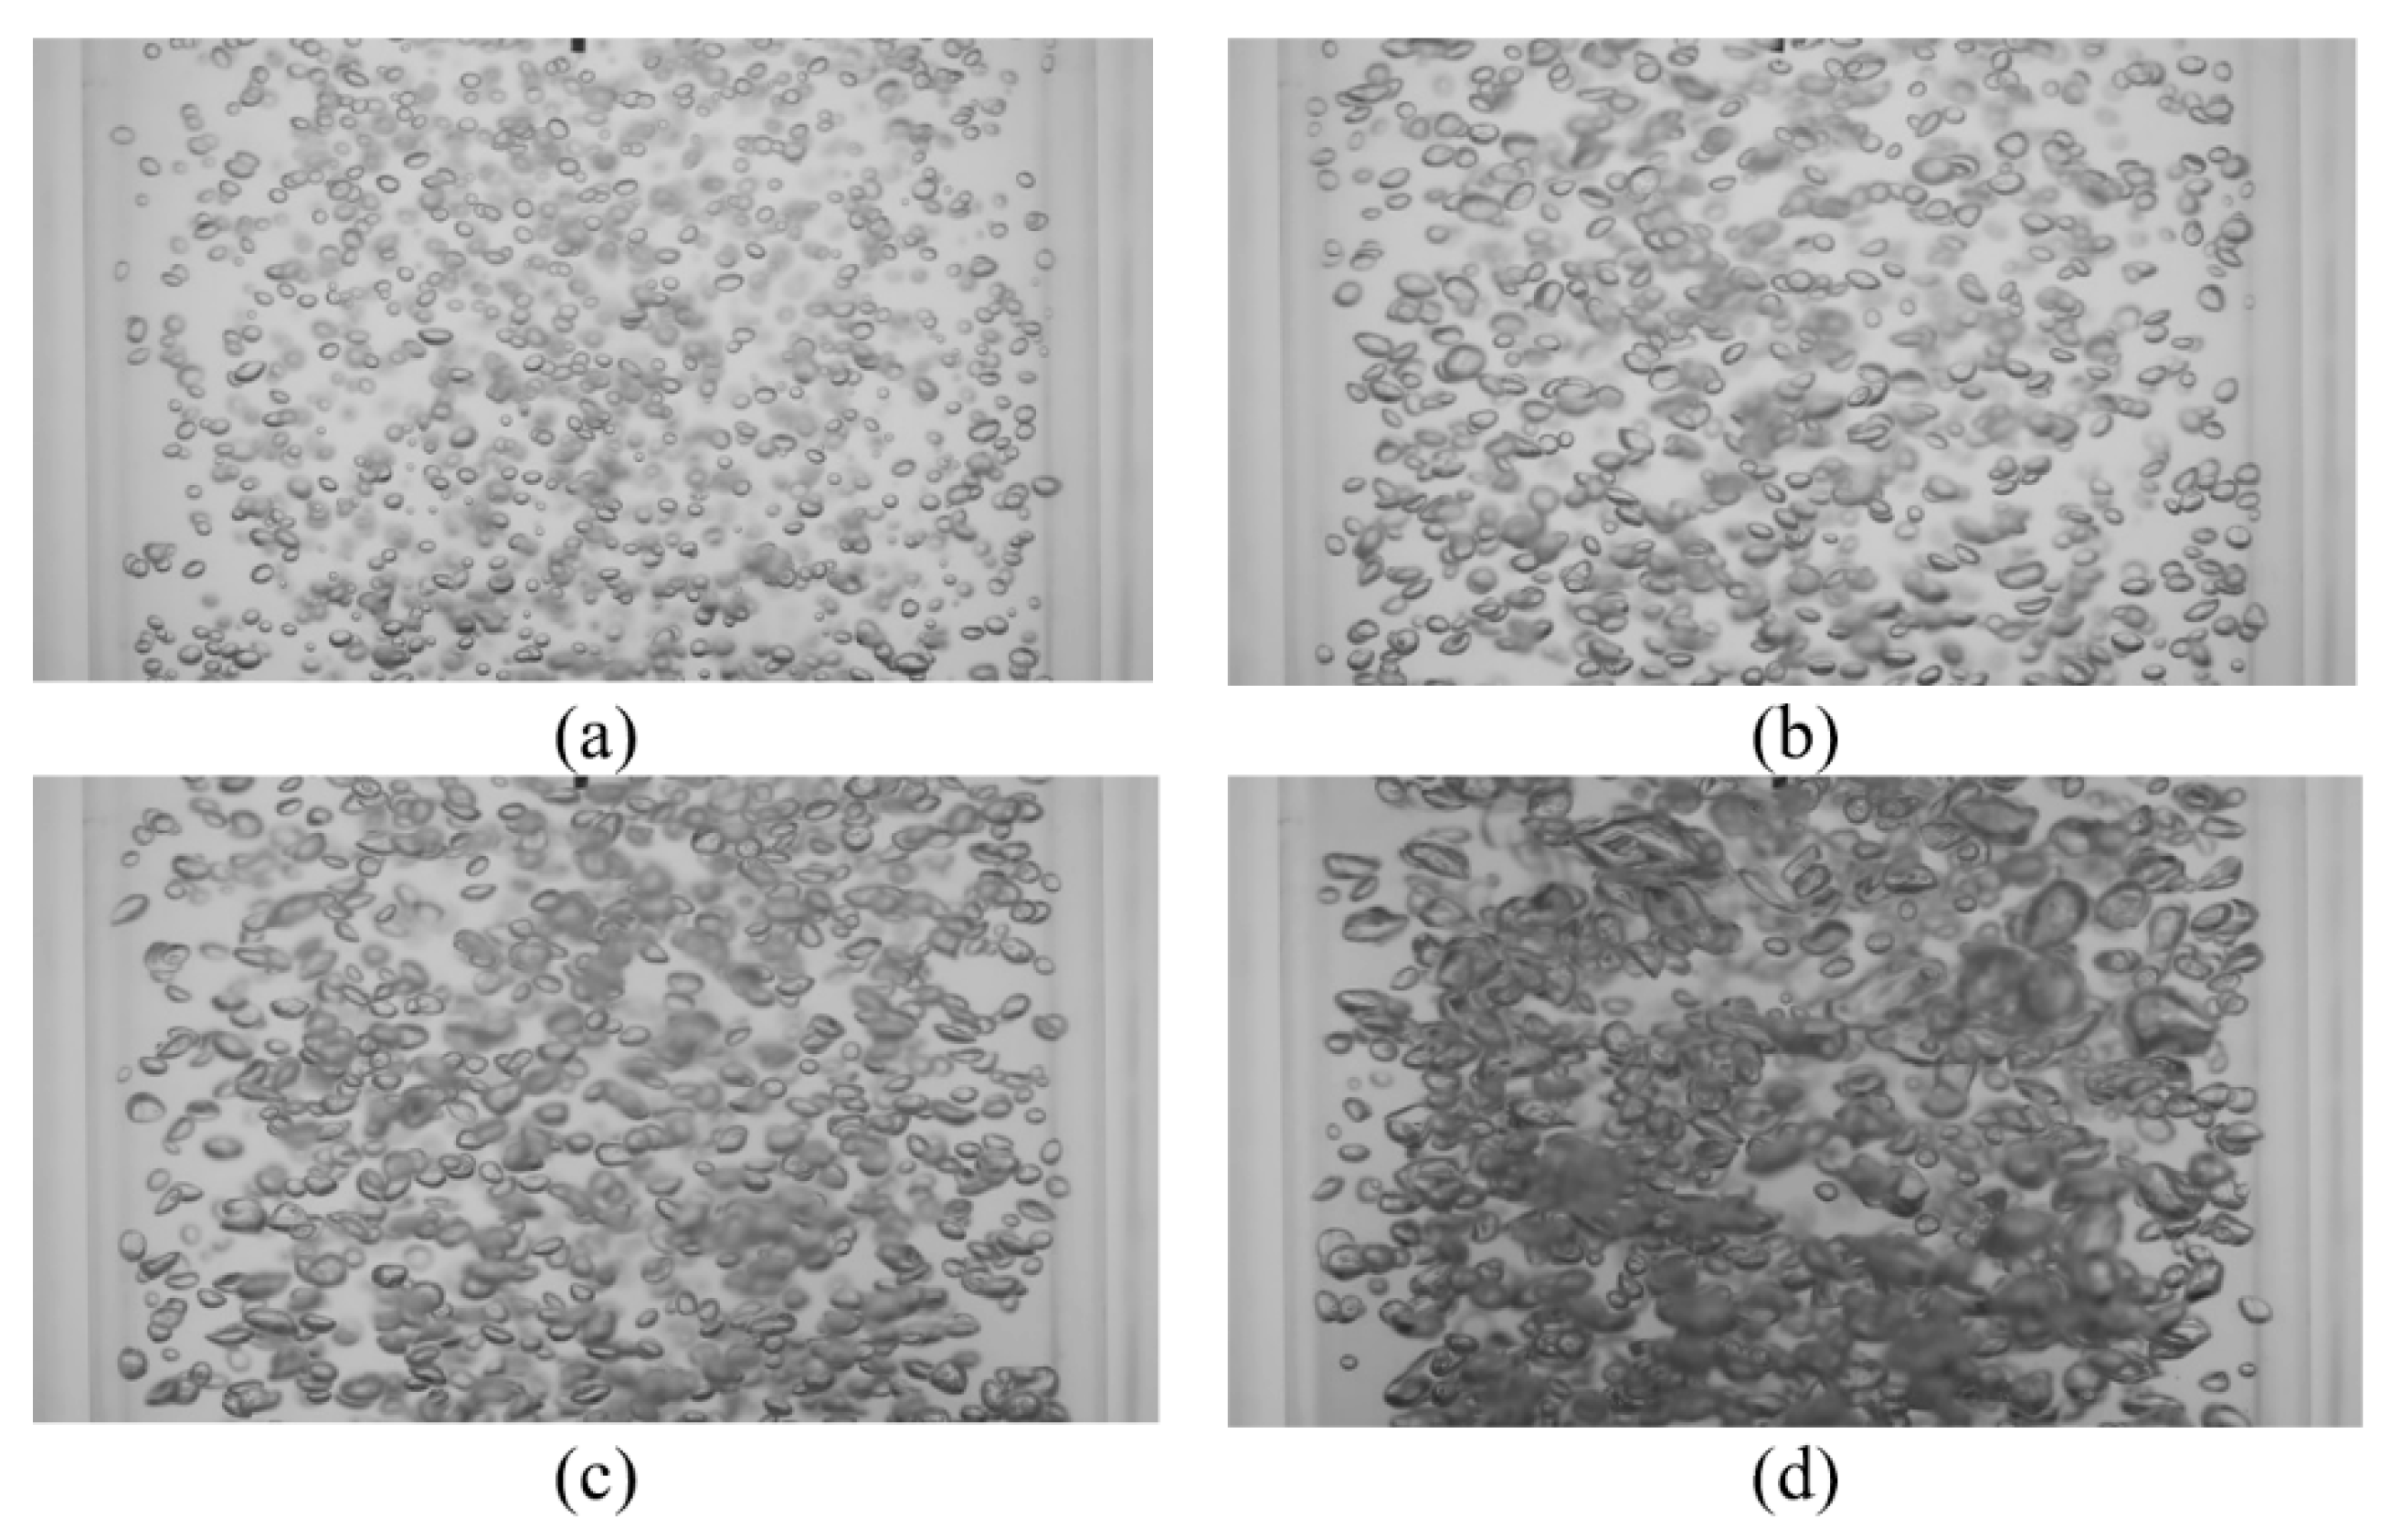
\includegraphics[width=4cm]{image/bubbles_2}
  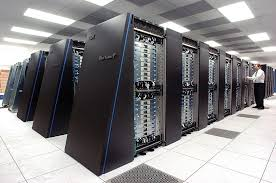
\includegraphics[width=4cm]{image/HPC}
\end{figure}
$\textcolor{orange}{\underbrace{ {\pSavg{{\left[\textbf{r}\bm{\sigma}_f' \cdot \textbf{n}-\mu_f(\textbf{u}_f'\textbf{n} +\textbf{n}\textbf{u}_f')\right]}}}}_\text{First moment} }$ cannot straightforwardly be measured in inertial flows ! 
\end{frame}




\section{Stresslet}
\section*{}





\begin{frame}{Stresslet}
  \small
\begin{equation*}
  %\underbrace{ {\pSavg{{\left[\textbf{r}\bm{\sigma}_f' \cdot \textbf{n}-\mu_f(\textbf{u}_f'\textbf{n} +\textbf{n}\textbf{u}_f')\right]}}}}
  \text{First moment}
  = 
  \underbrace{\pSavg{(\textbf{r}\bm{\sigma}_f' +\bm{\sigma}_f' \textbf{r} )\cdot \textbf{n}-\mu_f(\textbf{u}_f'\textbf{n} +\textbf{n}\textbf{u}_f')}}_{\text{Stresslet} (\bm S)}
  +
  \bm\epsilon \cdot \underbrace{\pSavg{\textbf{r} \times \bm{\sigma}_f' \cdot \textbf{n}}}_{\text{Torque} (\bm T)}
\end{equation*}

\setbeamercovered{transparent=10}
\only<1>{
  \centering
  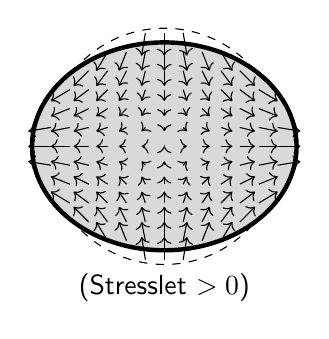
\begin{tikzpicture}[ultra thick,scale=0.6]
    \def\nRows{6}
    \def\nCols{6}
    \draw[dashed,thin] (0,0)circle(2.5);
    \draw[fill=gray!30] (0,0)ellipse(2.8 and 2.2);
    \foreach \x in {-\nRows,...,\nRows} {
        \foreach \y in {-\nCols,...,\nCols} {
            \pgfmathsetmacro\distance{veclen(\x*0.4, \y*0.4)};
            \pgfmathparse{\distance < 2.45 ? "blue" : "white"}
            \edef\colour{\pgfmathresult};
            \ifthenelse{\equal{\colour}{blue}}{                    
                \draw[thin,->](\x*0.4,\y*0.4)--++(0.08*\x,-0.08*\y);
            }
        }
    }
    \node (txt) at (0,-3){(Stresslet $> 0$)};
\end{tikzpicture}
\hspace{1em}
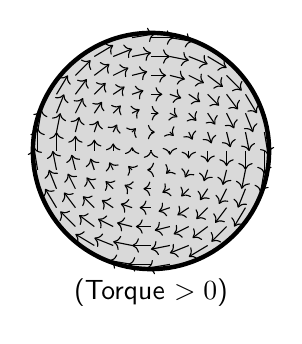
\begin{tikzpicture}[ultra thick,scale=0.6]
    \def\nRows{6}
    \def\nCols{6}
    \draw[fill=gray!30] (0,0)circle(2.5);
    \foreach \x in {-\nRows,...,\nRows} {
        \foreach \y in {-\nCols,...,\nCols} {
            \pgfmathsetmacro\distance{veclen(\x*0.4, \y*0.4)};
            \pgfmathparse{\distance < 2.5 ? "blue" : "white"}
            \edef\colour{\pgfmathresult};
            \ifthenelse{\equal{\colour}{blue}}{                    
                \draw[thin,->](\x*0.4,\y*0.4)--++(0.08*\y,-0.08*\x);
            }
        }
    }
    \node (txt) at (0,-3){(Torque $> 0$)};
\end{tikzpicture}
}
\only<2->{
\uncover<2>{\textbf{Shear dominated flows (Einstein 1906, Taylor 1932)}
\begin{equation*}
  \bm S
  = \frac{3}{5}\mu_f \phi \left(\frac{2+5\lambda}{1+\lambda}\right) \left(\grad \textbf{u}_f + ^\dagger \grad \textbf{u}_f\right)
  + \mathcal{O}(\phi^2, Re)
\end{equation*}
$Re$ correction only published in the early 2000 (Stone et al. 2001, Raja et al. 2010) !
%Thus, $\frac{3}{5}\phi \left(\frac{2+5\lambda}{1+\lambda}\right)$ it can be considered as an effective viscosity ! 
}

\uncover<3>{\textbf{Droplet in translation}
\begin{equation*}
  \bm S
  = \bm 0 + \mathcal{O}(\phi^2, Re)
\end{equation*}
%So the relative velocity doesn't contribute to the Stresslet  ? 

}

\uncover<4>{
  \textbf{We must consider the effect of finite $Re$  !}
}}
\end{frame}

%\section{Reciprocal theorem}

\section{Mathematical approach}
\begin{frame}
  \frametitle{History of the Reciprocal theorem}
\begin{figure}
  \centering
  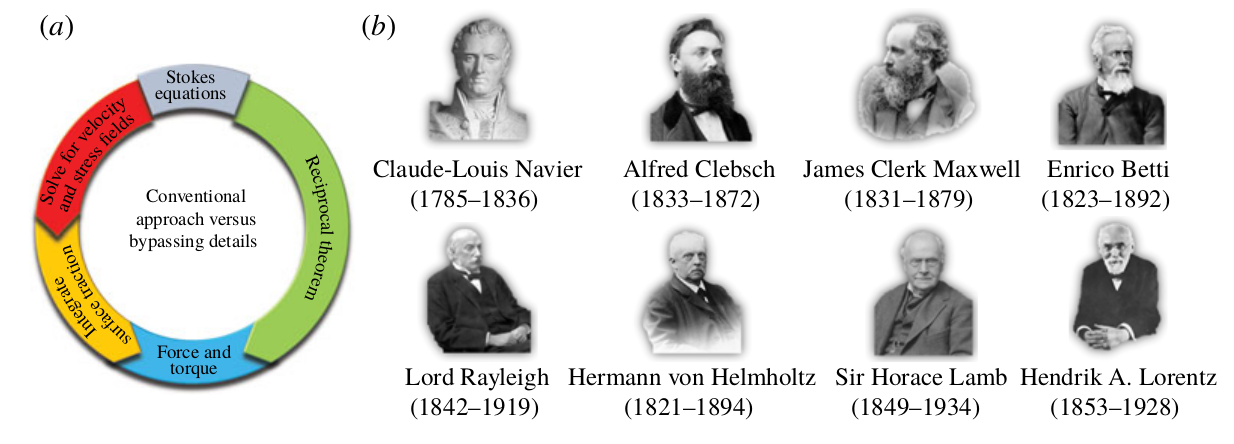
\includegraphics[width=12cm]{image/reciprocal_diag}
  \caption{From Massoud \& Stone (2018)}
\end{figure}

$...$ provide "something for nothing"
\end{frame}
 

\begin{frame}
  \frametitle{Reciprocal theorem}

Reciprocal theorem (Stone et al. 2001, Massoud et Stone 2019)
\begin{align}
  \div \bm v =& 0 \quad \div \boldsymbol{\sigma} = \bm f \\
  \div \hat{\bm v} =& 0 \quad \div \hat{\boldsymbol{\sigma}} =  \hat{\bm f} \quad \text{with same boundaries}
\end{align}
{\Huge Step \only<1>{1}\only<2>{2}\only<3->{3}:
}
\begin{equation*}
  \uncover<3->{\int_{V_f}\left\{ }
  \fbox{Equation of $\bm v$} \cdot \hat{\bm v} 
  \uncover<2->{
    - \fbox{Equation of $\hat{\bm v}$} \cdot  \bm v 
    }
  \uncover<3->{\right\}dV}
\end{equation*}
\begin{equation}
  \uncover<4->{\int_S \bm n \cdot \bm \sigma \cdot \hat{\bm v} dS - \int_S \bm n \cdot \hat{\bm \sigma} \cdot \bm v dS = \int_{V_f} \hat{\bm v}\cdot \bm  f dV - \int_{V_f} \bm v\cdot \bm  \hat{\bm f} dV}
  %\int_S \bm n \cdot \bm \sigma \cdot \hat{\bm v} dS - \int_S \bm n \cdot \hat{\bm \sigma} \cdot \bm v dS = \int_{V_f} \hat{\bm v}\cdot \bm  f dV - \int_{V_f} \bm v\cdot \bm  \hat{\bm f} dV
\end{equation}
\end{frame}


\begin{frame}
  \frametitle{Test problem and regular expansion in $Re$}
  %{Regular expansion in $Re$ }

  True problem (pure translation): $\textbf{u}_r  = \textbf{u}_r|_{\bm x = \bm x_p} = \textbf{u}_f-\textbf{u}_p$
  \vspace{0.5cm}

  Test problem 
  \begin{itemize}
    \item linear flow (stokes regime) : $\hat{\textbf{u}_r} =  \textbf{r} \cdot \nabla \hat{\textbf{u}}_f |_{\bm x = \bm x_p}$
    \item point source solution (stokes regime)
  \end{itemize}
  \vspace{0.5cm}

  Assuming small but finite $Re$ : $\bm f = \bm f^{(0)} + Re  \bm f^{(1)} + Re^2  \bm f^{(2)} + \ldots$. 

  
  \begin{equation*}
    \bm f^{(0)}
    =
        \pddt \bm v^{(0)}
        + \bm v^{(0)}\cdot \grad\bm v^{(0)} 
        +  \bm v^{(0)}\cdot \grad\textbf{u}_r 
        +  \textbf{u}_r\cdot \grad\bm v^{(0)}
  \end{equation*}

  $\to$ $\bm v^{(0)}$ is governed by the Stokes equation this is thus a known field ! 
  \uncover<2>{
  \begin{equation}
      Re \intOf{\hat{\bm v} \cdot  \bm f}
      =
      Re \intOf{\hat{\bm v} \cdot  \bm f^{(0)}}
      + \mathcal{O}(Re^2)
    \end{equation}
    }
\end{frame}

%\section{Inertial stresslet}
%\section*{}

\begin{frame}
  \frametitle{Inertial stresslet due to the relative motion of droplets}
\setbeamercovered{transparent=15}


  \begin{align*}
    \frac{a}{\mu_f u_r} \bm S
    % \left[
        %\pSavg{\textbf{r}\bm{\sigma}_f^0 \cdot \textbf{n}}
        %\pSavg{(\textbf{r}\bm{\sigma}_f^0 +\bm{\sigma}_f^0 \textbf{r} )\cdot \textbf{n}-\mu_f(\textbf{u}_f'\textbf{n} +\textbf{n}\textbf{u}_f')}\\
        % - \pOavg{(2 \mu_f \textbf{e}_d^0 - p_f\bm\delta)}
        % \right]
        % \\
     =
    \phi Re C_1
    [
      \textbf{u}_r\textbf{u}_r - \frac{1}{3}u_r ^2\bm\delta 
      ]
      + Re \phi C_2 (u_r ^2) \bm\delta
      % + \phi p_f \bm\delta
  \end{align*} 
\begin{align*}
    C_1  =  -\frac{63 \lambda^{3} + 150 \lambda^{2} + 112 \lambda + 28}{80 \left(\lambda + 1\right)^{3}}
    &&
    C_2  = \frac{3\lambda^2 + 6\lambda + 4}{48(\lambda +1 )^2}
  \end{align*}
  
For rising suspension in one direction : normal stress difference $\propto C_1 \bm u_r^2$.
$\to$ rising droplets deform in oblate spheroid when $Re > 0$ (Taylor \& Acrivos 1964)%due to the non-zero Stresslet (Taylor \& Acrivos 1964)!
  %\begin{itemize}
  % \item 
  %  \item 

    %\item \textbf{U}=$\textbf{u}_p-\textbf{u}_f$ Mean relative velocity between phases
%  \end{itemize}
%  $\to$ Rising droplets deform when $Re > 0$ due to the non-zero Stresslet (Taylor \& Acrivos 1964)!

\end{frame}





%\begin{itemize}

%\end{itemize}
\section{Inertial rheology}
\section*{}

\begin{frame}
  \frametitle{Effective stress in rising suspension}
  \setbeamercovered{transparent=15}
    \begin{equation*}
      \phi_f \rho_f (\pddt + \textbf{u}_f\cdot \grad)\textbf{u}_f
      = 
      \phi_f \div \bm\Sigma^\text{f} +
      \div \bm\sigma^\text{eff}
      + \phi_f \rho_f \textbf{g} 
      - \pSavg{{\bm{\sigma}_f' \cdot \textbf{n}}}
  \end{equation*}
  \underline{Assuming $\grad \textbf{u}_f = 0$ :}
  \begin{align*}
    \frac{a }{\mu_f u_r}\bm{\sigma}^\text{eff}_f 
    &=\frac{a }{\mu_f u_r} \left(
      \bm S -  \avg{\chi_f\rho_f\textbf{u}_f'\textbf{u}_f'} \right)
    \\
    \uncover<2>{&= 
    \left[Re \phi  ( C_2-C^{Re}_2)(\textbf{u}_r\cdot \textbf{u}_r) \right]\bm\delta 
    + Re \phi ( C_1 - C^{Re}_1)\left[
            \textbf{u}_r\textbf{u}_r
            - \frac{1}{3}(\textbf{u}_r\cdot \textbf{u}_r)\bm\delta
    \right]}
    % + \mathcal{O}(Re^{3/2},\phi^2).
    \label{eq:stress_closed}
\end{align*} 
%\uncover<2>{
%$C_1$ valid only for $\boxed{\phi \ll 1}$ and $\boxed{Re < 1}$
%$\longrightarrow$
%\textbf{DNS measurements ! }
%}
\end{frame}

\begin{frame}
  \frametitle{Direct Numerical Simulations of rising droplet suspension}
  \begin{columns}
    \column{0.6\textwidth}
    \only<1>{
    \underline{Simulation set up:} 
  \begin{itemize}
  \item Tri-periodic boundary conditions.
  \item Buoyancy only.
  \item \textbf{Mono-disperse} distribution of droplet size.
  \item We prevent (VOF) coalescence using a special algorithm 
    (\href{http://basilisk.fr/src/no-coalescence.h}{no-coalescence.h})
  \item Free Software: \url{http://basilisk.fr}
  \end{itemize}
  }
  \only<2>{
    \underline{Energy consumptions} 
    \begin{itemize}
 \item Each simulation : 512 cores during 48 hours
 
 \item 1 core consumption:  $\sim 5$ W

 \item Energy comsumption for each run : $\sim 100$ kWh $\sim 200 $km with a Clio
\end{itemize}
  %\begin{itemize}
  %  \item \textit{Galileo} number: $Ga =\frac{\sqrt{\rho_f \Delta\rho_f gD^3}}{\mu} \in [5, 100]$
  %  \item \textit{Bond} number: $Bo = \frac{\Delta \rho_f g D^2}{\sigma} = 0.2$ 
  %  \item Volume fraction of dispersed phase: $\phi = [0.01;0.2]$. 
  %  \item Density and viscosity ratio, $\zeta=\rho_d/\rho_f=0.9$ and $\lambda=\mu_d/\mu_f= 10,1,0.1$. 
  %\end{itemize}
  }
  \vfill
  % \begin{figure}
  %  \caption{Snapshot of a simulation at $T_g = 300$ for $\phi = 0.01$, $Ga = 75$, $\mu_r = 0.1$ and $N_b = 125$. In white, the interfaces ; the background color map corresponds to the pressure field. The grid represents the different parallel cores.
  %  }
  % \end{figure}
  \column{0.5\textwidth}
  \centering
  \href{videos/DNS.mp4}{\beamergotobutton{Play}}
  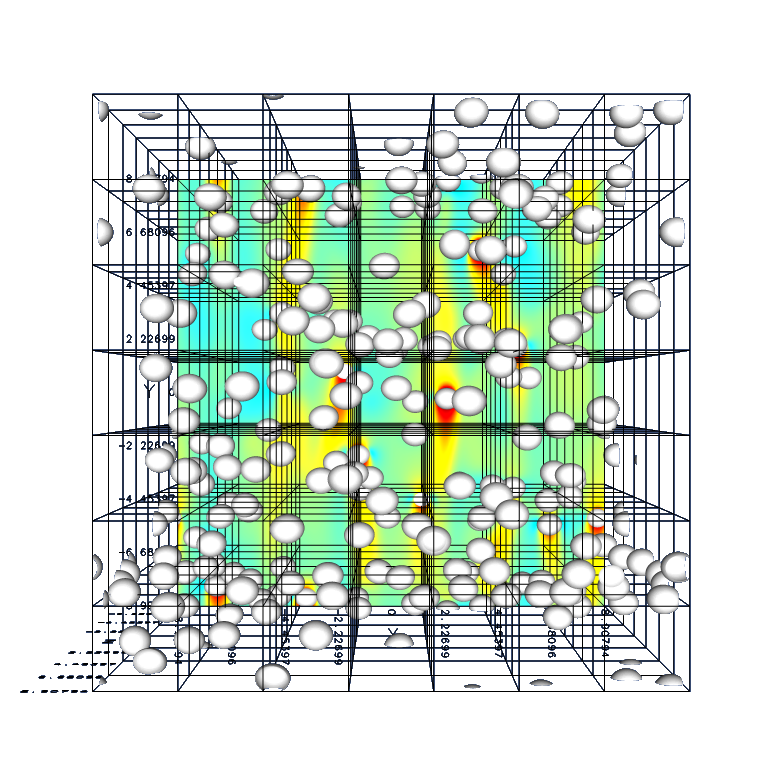
\includegraphics[width =  \textwidth]{image/PHI_01_Ga_75.png}

  \end{columns}
\end{frame}

\begin{frame}
  \begin{figure}[h!]
    \centering
    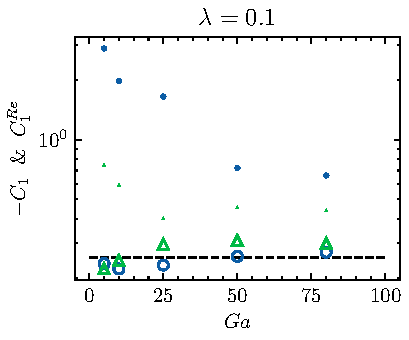
\includegraphics[height = 0.25\textwidth]{image/HOMOGENEOUS_final/PA/Sdev_diapo_l_1.pdf}
    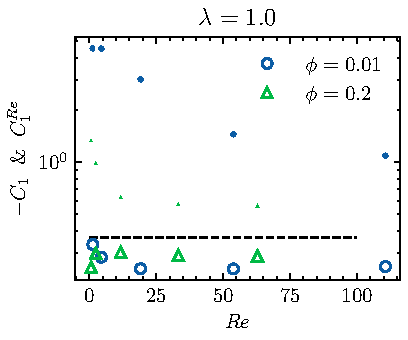
\includegraphics[height = 0.25\textwidth]{image/HOMOGENEOUS_final/PA/Sdev_diapo_l_10.pdf}
    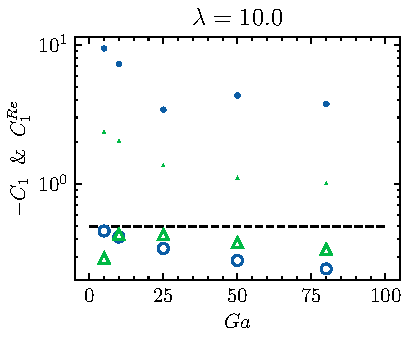
\includegraphics[height = 0.25\textwidth]{image/HOMOGENEOUS_final/PA/Sdev_diapo_l_100.pdf}
    \caption{
      (Hollow symbols) \underline{Stresslet}: $C_1$. 
      (Filled symbols) \underline{Reynolds stress} $C_1^{Re}$. 
     }
\end{figure}
\begin{itemize}
\item $\phi \ll 1$ : $\avg{\chi_f\rho_f\textbf{u}_f'\textbf{u}_f'}\propto \phi^{2/3}$ while $\bm S \propto \phi \rightarrow$   $\avg{\chi_f\rho_f\textbf{u}_f'\textbf{u}_f'}\gg \bm S$
\item $\phi \approx 0.2$ : $\avg{\chi_f\rho_f\textbf{u}_f'\textbf{u}_f'}\sim \bm S$
\end{itemize}
%\item $\avg{\chi_f\rho_f\textbf{u}_f'\textbf{u}_f'}$ $\gg$ Stresslet for $\phi \ll 1$ %\item Good trends in terms of $\sim \phi^{2/3}$ and $\lambda$.  
%\item Quantitative agreement for $\phi < 0.01$.  
\end{frame}

\section{Discussion and perspectives}
\section*{}






\begin{frame}
  \frametitle{Discussion}
  %\centering
  %{\Huge\textbf{Discussion and perspectives ? }}
 %Lin et al. (1970), Stone et al. (2001), Raja et al. (2010) derived the first correction to Einstein-Taylor viscosity for ($Re_{\dot{\gamma}}\ll 1$):

% \begin{equation}
%\bm S = \frac{3}{5}\mu_f \phi \left(\frac{2+5\lambda}{1+\lambda}\right) \left(\grad \textbf{u}_f + ^\dagger \grad \textbf{u}_f\right) + \color{orange}Re_{\dot{\gamma}}\left(...\right)
%\end{equation}
Shear induced rheology:
 \begin{equation}
\bm\sigma^\text{eff} =  \mu_\text{eff} \left(\grad \textbf{u}_f + ^\dagger \grad \textbf{u}_f\right) \propto \mu_\text{eff} \dot{\gamma}
\end{equation}

Relative velocity rheology:
\begin{equation}
  \bm\sigma^\text{eff}
  \propto \rho_f u_r^2
\end{equation}

\begin{equation}
  \rho_f \textbf{u}_r \textbf{u}_r \gg \mu_\text{eff} \left(\grad \textbf{u}_f + ^\dagger \grad \textbf{u}_f\right) \Leftrightarrow Ga \gg \frac{\dot{\gamma}\mu_{eff}}{(\rho_d-\rho_f)g a}
\end{equation}

An assumption which is satisfied in pipe flow (far from the wall) for most of the inclusions encountered in processes.%pipe laminar flow and most probably in turbulent flows far from the wall for most of the inclusions. 
 %However, in buoyancy driven flows the $Re_{\dot{\gamma}}$ correction is  negligible if $u_r \gg a\dot{\gamma}$ which leads to (for dilute sedimenting suspension),

 %\begin{equation}
 % \frac{\rho _p}{\rho_f} \gg 1 + \frac{9}{2} \frac{\dot{\gamma}\mu}{a \rho _f g}
 %\end{equation}
%For solid particles in gas or bubbles in liquids we may expect the $Re_{\dot\gamma}$ correction to be negligible
 
\end{frame}

\begin{frame}
  \frametitle{Discussion}
  \begin{itemize}
    \item Theoretical approaches can be as effective and insightful as modern CFD simulations  
    \item Progress in the study of dispersed two-phase is very long
  \end{itemize}
%  \begin{itemize}
%    \item Dispersed phase equations : center of mass velocity variance ?
%    \item How to measure the coefficient $C_1$ and $C_2$ with experiments  ?
%    \item Does the system of equations is hyperbolic ? %With effective stress $\propto U^2$ ?
%    \item Do the proposed closures laws agree with rheological principles (material objectivity, etc) ?
%  \end{itemize}
\end{frame}


\backmatter

%\begin{frame}
%  \footnotesize

%  \bibliography{Bib/bib_bulles.bib}

%\end{frame}

\begin{frame}
  \frametitle{Reformulation of the first moment  with conditional average}
  
    \begin{equation*}
      \underbrace{\pSavg{{\textbf{r} \bm{\sigma}_f^0 \cdot \textbf{n}}}[\textbf{x},t]}_\text{$N$ droplets in a fluid}
      =
      \underbrace{n_p[\textbf{x},t]
        \intS[]{\textbf{r} \bm\sigma^1 \cdot \textbf{n}}}_\text{
        \href{videos/one_particle.mp4}{One droplet in an effective medium}
        }
    \end{equation*}
  \begin{itemize}
    \item $\bm\sigma^1[\textbf{z}|\textbf{x}]$ Mean stress at \textbf{z} conditioned on the presence of a droplet at $\textbf{x}$. 
  \end{itemize} 
  \vfill
  $\to$ This time we need a result of $\bm\sigma$ accurate at $\mathcal{O}(Re)$. 
\end{frame}



\begin{frame}
  \frametitle{Why the 'outer solution' is negligible to leading order ?}
  \begin{equation}
    \int _{V_f}\hat{\bm v} \cdot \bm f^{(0)} d\Omega= \int _{V_f}\hat{\bm v}\cdot(\textbf{u}_r\cdot\grad \bm v^{(0)}) d\Omega
  \end{equation}
  Since $\textbf{u}_r\sim \mathcal{O}(1)$, $\bm v^{(0)}\sim \mathcal{O}(r^{-1})$, $\hat{\bm v} \sim r^{-2}$ (linear flow pertubation) hence 
  \begin{equation}
    \hat{\bm v}\cdot(\textbf{u}_r\cdot\grad \bm v^{(0)}) = r^{-4},
  \end{equation}
  Additionally, the Oseen outer solution dominates over form $|\textbf{r}| > Re^{-1}$ to $|\textbf{r}|\to \infty$ for a droplet in translation.
  Consequently, the outer solution contribution to the first moment is given by, 
  \begin{equation}
      \lim_{Re \to 0 }
      \int_{Re^{-1}}^\infty
      \hat{\bm v}\cdot(\textbf{u}_r\cdot\grad \bm v^{(0)})
      d\Omega
      =
      \lim_{Re \to 0 }
      \int_{Re^{-1}}^\infty
      \mathcal{O}(r^{-2})
      dr
      = \mathcal{O}(Re). 
  \end{equation}
  %Since this term is already factor of $Re$ in the expression of the first moment we are allowed to neglect the outer field contribution. 
  Consequently, the regular perturbation is accurate with an error of $\mathcal{O}(Re^2)$. 
\end{frame}

\begin{frame}
  \frametitle{How to compute the first moment within the DNS ?}

  \underline{Steady state} first moment of momentum equation:
  \begin{multline*}
    \pSavg[i]{\textbf{r}\bm\sigma_f^0\cdot \textbf{n}}
    = 
    \underbrace{- \pOavg[i]{\rho_d \textbf{w}_d^0  \textbf{w}_d^0 }
    + \pOavg[i]{\bm\sigma_d^0}}_\text{volume integrals}\\
    +  \underbrace{\gamma \pSavg[i]{(\bm\delta - \textbf{nn})}}_\text{Geometry of the surface}
\end{multline*}

\uncover<2>{$\to$ We are thus able to meusure $C_1$ (and $C^{Re}_1$) from DNS !}
\end{frame}






\begin{frame}{Comparison with Particle Resolved Simulations (PRS)}
  \begin{figure}[h!]
    \centering
    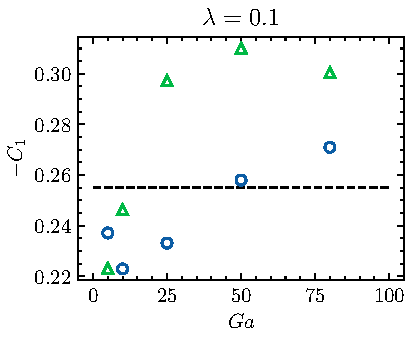
\includegraphics[height = 0.25\textwidth]{image/HOMOGENEOUS_final/PA/Sdev_diapo2_l_1.pdf}
    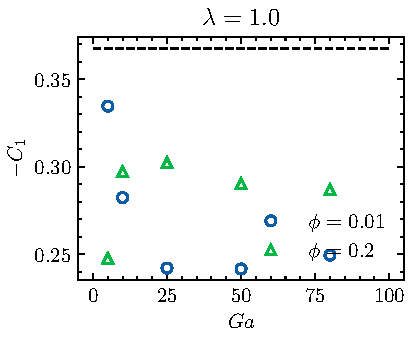
\includegraphics[height = 0.25\textwidth]{image/HOMOGENEOUS_final/PA/Sdev_diapo2_l_10.pdf}
    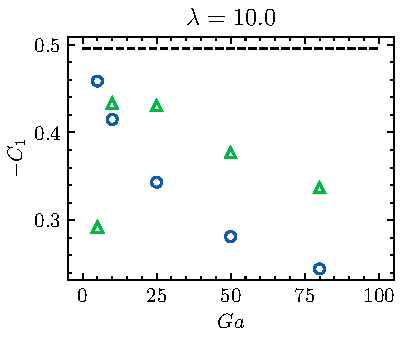
\includegraphics[height = 0.25\textwidth]{image/HOMOGENEOUS_final/PA/Sdev_diapo2_l_100.pdf}
    \caption{$--$ : theoretical prediction, points : PRS.  Viscosity ratio ($\lambda =$). 
      %(Hollow symbols) \underline{Stresslet}: $C_1$. 
      %(Filled symbols) \underline{Reynolds stress} $C_1^{Re}$. 
     }
\end{figure}

The theoretical formula gives the correct order of magnitude (and correct sign).
%\uncover<2>{
%\textbf{In dense regime the Stresslet may not be negligible !}
%}


\end{frame}


\begin{frame}
  \frametitle{Experiments and PRS results}
  \begin{figure}[h!]
    \centering    
    % 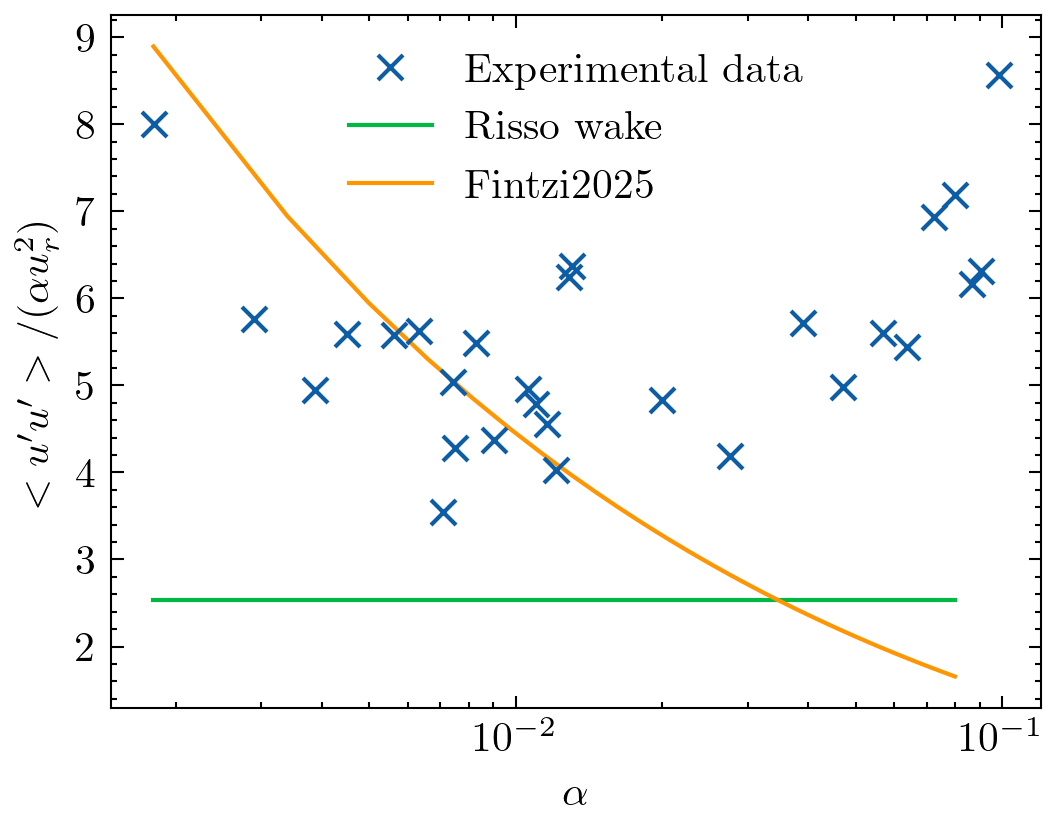
\includegraphics[height = 0.25\textwidth]{image/upupexp.png}
    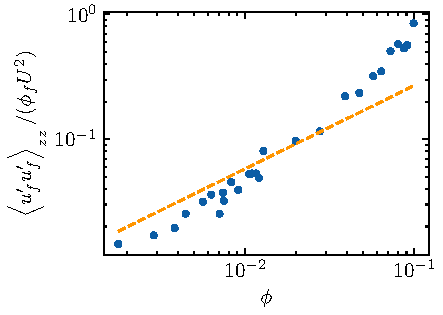
\includegraphics[height = 0.20\textwidth]{image/HOMOGENEOUS_final/CA/cartellier.pdf}
    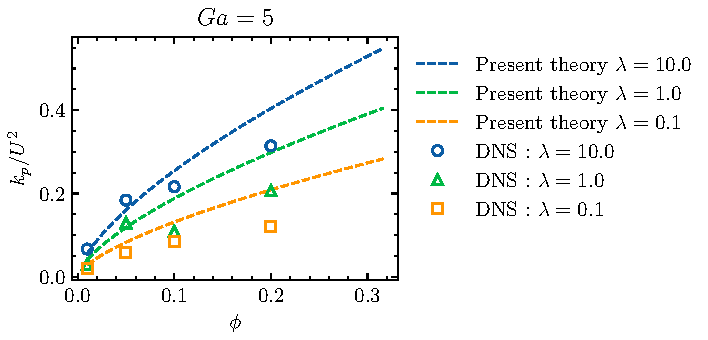
\includegraphics[height = 0.20\textwidth]{image/HOMOGENEOUS_final/CA/UUyy_Ga_5.pdf}
    \caption{
      %  Dimensionless vertical component of the Reynolds stress :
      (left) Comparison with the rising bubbles experiment of Cartellier \& Riviere with $Re \approx 10$.
      (right) comparison with DNS for two viscosity ratio $\lambda =1,10$ and $Re \approx 1$ DNS. 
        
    }
\end{figure}  
\end{frame}


\begin{frame}
  \frametitle{Buoyancy driven two-fluid rheology}
  \centering\underline{Continuous phase mass and momentum equation:}
  \begin{equation*}
    \pddt \phi_f + \div (\textbf{u}_f \phi_f) = 0
  \end{equation*}
  \begin{equation*}
    % \pddt \phi_f + \div (\textbf{u}_f \phi_f) &= 0\\ 
      \rho_f (\pddt 
    + \textbf{u}_f \cdot \grad)
    \textbf{u}_f
    = 
    \div\bm\Sigma_f
    % \underbrace{\div\bm\Sigma_f}_\text{Newtonian stress}
    + \rho_f \textbf{g}
    \only<2->{\textcolor{sintefcyan}{-\underbrace{C_D(Re,\phi, \lambda) \frac{3}{8} \frac{\rho_f}{a}  \frac{\phi}{1-\phi}   \times \textbf{u}_r |\textbf{u}_r|}_\text{Drag force}}}
    \only<3>{\textcolor{sintefred}{+\underbrace{\frac{1}{1-\phi} \div  \bm{\sigma}_f^{\text{eff}}}_\text{Effective stress}}}
  \end{equation*}

  \centering\underline{Constitutive laws:}

\begin{equation*}
    \bm\Sigma_f 
    = 
    - p_f \bm\delta
    + 2\mu_f \left[\grad \textbf{u}_f + (\grad \textbf{u}_f)^\dagger\right]
\end{equation*}

\uncover<3>{
\begin{equation*}
\textcolor{sintefred}{
    \bm{\sigma}^{\text{eff}}_f 
    = \underbrace{C_E(Re,\phi,\lambda) \mu_f [\grad \textbf{u}_f +  (\grad \textbf{u}_f)^\dagger ] }_\text{``Einstein viscosity''}% \& Single phase Turbulence}
    + 
    \underbrace{
      A_{u_r}(\phi,\lambda,Re)\textbf{u}_r\textbf{u}_r
    + B_{u_r}(\phi,\lambda,Re)u_r^2 \bm\delta}_\text{Fluid velocity variance \& Stresslet}
}
\end{equation*}
}

\end{frame}







\end{document}
